\subsection{Results (proto v2)}

An additional set of accuracy measurements were taken with GIAANN Proto 2.

A number of changes to the default settings were introduced in GIAANN Proto 2 that affect evaluation accuracies (\texttt{useDefaultsV2}):

\subsection{proto v2j+ settings}
\begin{itemize}
 	\item Implement option tokeniserSubword - a modern BPE/SentencePiece subword tokeniser (\texttt{o200k_base} encoding of the OpenAI \texttt{tiktoken} library \citep{openai2022tiktoken}).
    \item Implement option \texttt{SANIcolumnsLinkFirstSegmentToAllPriorTrainSeqTokens=False}, which affects both \texttt{useSANIfeaturesAndColumns} and \texttt{useSANIcolumns} modes.
    \item Enable option \texttt{SANIfeaturesLinkFirstSegmentToAllPriorTrainSeqTokens=False}, which affects both \texttt{useSANIfeaturesAndColumns} and \texttt{useSANIfeatures} modes.
    \item Restore \texttt{inferenceBurstAllPredictionsOrTargetsInSequence} - patch inference to always activate the top-1 selected feature neuron (i.e. the prediction or target respectively as per \texttt{inferenceUseNextTokenPredictionsOrTargetsToActivateNextColumnFeatures}). This guarantees the selected top-1 feature is active when the next step uses it as a source.
\end{itemize}

\subsection{proto v2k+ settings}
\begin{itemize}
	\item update \texttt{inferenceEvaluateTestSetTrainMaxSequences10M}. Eval datasets contain 1000 sequences, and were extracted to support 10M training sequences. set \texttt{inferenceEvaluateTestSetTrainMaxSequences10M=True}.
	\item set \texttt{inferenceDecrementActivations=True} and \texttt{activationDecrementPerPredictedToken=0.05}
	\item set \texttt{inferenceActivationsType = "intf+c"} (required with inferenceDecrementActivations).
	\item add option \texttt{inferenceSegmentTimingMultipicativeBias=True} that affects option \texttt{inferenceSegmentTiming="biased"} only. Set \texttt{inferenceSegmentTiming="biased"}.
	\item set \texttt{SANIfeaturesAndColumnsDistribution=="matchedSegments"} (equal number of feature and column segments).
	\item set \texttt{skipSequenceNoDelimiterDetectedBetweenConceptTokens==False}.
	\item enable \texttt{multisentencePredictions} and \texttt{sequencesCropToMaxLength}.
\end{itemize}

\subsection{proto v2m+ settings}
\begin{itemize}
    \item set \texttt{inferenceLeakyIntegrateAndFire=True} by default
    \item add option \texttt{inferencePromptPreserveLineSequenceBoundaries} - process each non-empty inference prompt line as exactly one independent sequence matching the stored training boundary
    \item add option \texttt{inferenceColumnConstraintsAllowExternalPrimeConceptTransitions} - allow external prime-concept candidates at no-delimiter column transitions without relabelling rejected candidates
\end{itemize}

\subsection{proto v2n+ settings}
\begin{itemize}
	\item  patch LIF implementation - take the max across all branches (do not sum branch activations).
	\item  set \texttt{inferenceDeactivateLastColumnSegmentUponPrediction=True} by default
	\item  add option \texttt{inferenceColumnConstraintsAllowExternalPrimeConceptTransitionsBeamCandiateFilteringPatch=True}: patch beam candidate filtering to respect \texttt{inferenceColumnConstraintsAllowExternalPrimeConceptTransitions} by using \texttt{constraintAllowsNode} in \texttt{selectTopInstanceNodesByActivation} and \texttt{buildInstanceColumnData}.
	\item  add option \texttt{inferenceConstraintAllowsNodeDelimiterFilteringPermitValidSameColumnContinuationsPatch=True}: patch \texttt{constraintAllowsNode} delimiter-mode filtering to permit valid same-column continuation features after reference-set delimiters.
\end{itemize}

\subsection{proto v2o+ settings}
\begin{itemize}
	\item add option \texttt{inferenceReviewPatch5BinaryTreeSomaProjection} (enabled) - combine the maximum terminal-column branch signal with the binary-tree soma signal for LIF scoring.
	\item add option \texttt{inferenceReviewPatch7AuxiliaryDirectSegment} (enabled) - read LIF direct connections from the soma coordinate when generating automatic word-similarity data, requiring regeneration of existing similarity data.
	\item add option \texttt{inferenceReviewPatch8ReuseObservedColumns} (enabled) - reuse already loaded observed columns after checking their feature-array sizes to avoid redundant database loading.
	\item add option \texttt{inferenceReviewPatch9LocalSourceActivation} (enabled) - restrict soma and branch activation reductions to the requested source neuron to reduce inference lookup work.
	\item add option \texttt{inferenceReviewPatch10LinearNeuronReset} (enabled) - reset LIF neuron activations using vectorised neuron and segment masks across branches to avoid pairwise coordinate comparisons.
	\item add option \texttt{inferenceReviewPatch11ProspectiveColumnScoring} (enabled) - score external-column LIF candidates using their prospective column-transition activations while preserving current-column scores and the live activation state.
	\item add option \texttt{inferenceReviewPatch12RetainContextWithoutOutgoingSource} (disabled) - retain newly arriving LIF context when the source connectivity lookup is empty and filter valid context candidates before top-K selection.
	\item add option \texttt{inferenceReviewPatch13poolTransitionsFromSimilarFeatures} (disabled) - if source neuron has no outgoing connections, pool transitions from features of same f index in different columns.
	\item add option \texttt{inferenceReviewPatch14NormaliseConnectionInputs} - normalise each exact source neuron's outgoing weights per target segment; preserves direct connectivity
\end{itemize}

\Cref{fig:protov2j-oscar-top1-accuracy-spacyPipelineOptimisations-inferenceConnectionStrengthTypes} graphs the v2j training-set and test-set eval results. Note the v2j test-set accuracies are significantly higher than v2k+ due to usage of the different (smaller v1) eval datasets (\texttt{inferenceEvaluateTestSetTrainMaxSequences10M=False}).

Three sets of v2o results are reported. Both \#1 and \#3 break the strict direct connectivity requirement during inference (\texttt{enforceDirectConnectionsSANI}), facilitating the estimation of transitions without previously seeing them (and therefore hallucinated transitions);

\begin{itemize}
      \item default: \texttt{inferenceReviewPatch12RetainContextWithoutOutgoingSource} only.
      \item \texttt{predictionEnsureConnectedToPreviousPrediction=True}: \texttt{inferenceReviewPatch14NormaliseConnectionInputs} only.
      \item \texttt{predictionEnsureConnectedToPreviousPrediction=False}: \texttt{inferenceReviewPatch12RetainContextWithoutOutgoingSource}, \texttt{inferenceReviewPatch13poolTransitionsFromSimilarFeatures}, \texttt{inferenceReviewPatch14NormaliseConnectionInputs}.
\end{itemize}

\Cref{fig:protov2o-oscar-top1-accuracy-spacyPipelineOptimisations-inferenceConnectionStrengthTypes} graphs the v2o training-set and test-set eval results. Note the test-set accuracies are dependent on the eval test-set dataset and context window size. Proto v2k+ uses larger eval datasets of approximately 1000 sequences (\texttt{inferenceEvaluateTestSetTrainMaxSequences10M=True}).

\clearpage

\begin{figure}[p]
      \centering
      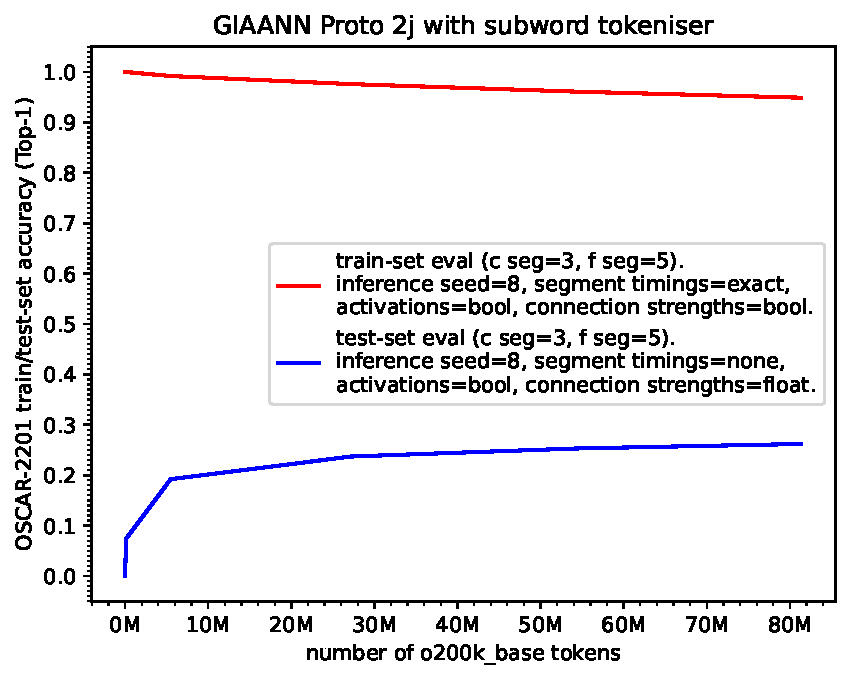
\includegraphics[width=0.80\linewidth]{graphs/protov2j-oscar-top1-accuracy-spacyPipelineOptimisations-inferenceConnectionStrengthTypes.pdf}
      \caption{GIAANN Proto 2j training-set and test-set accuracy.}
      \label{fig:protov2j-oscar-top1-accuracy-spacyPipelineOptimisations-inferenceConnectionStrengthTypes}
\end{figure}

\begin{figure}[p]
      \centering
      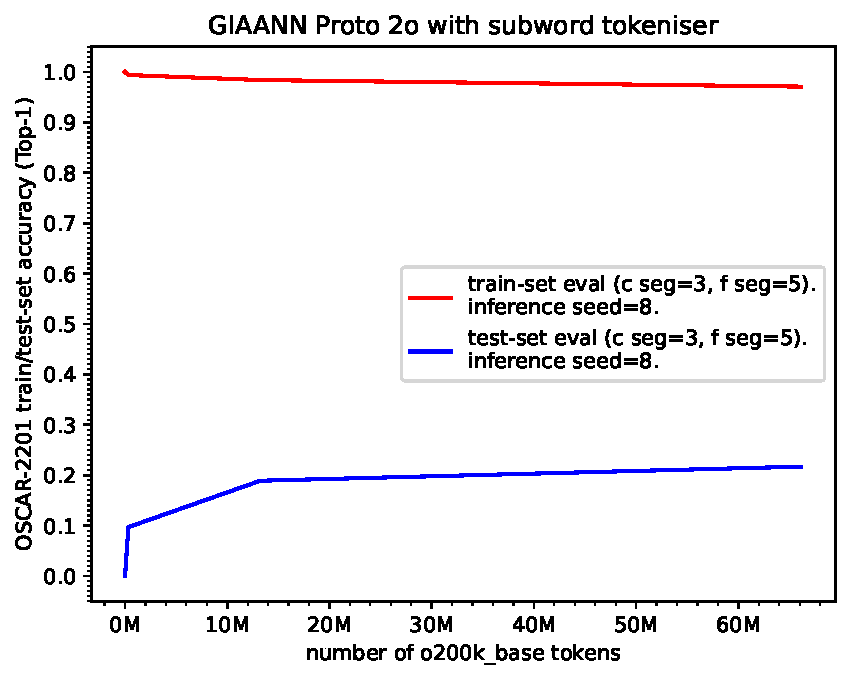
\includegraphics[width=0.80\linewidth]{graphs/protov2o-oscar-top1-accuracy-spacyPipelineOptimisations-inferenceConnectionStrengthTypes.pdf}
      \caption{GIAANN Proto 2o training-set and test-set accuracy.}
      \label{fig:protov2o-oscar-top1-accuracy-spacyPipelineOptimisations-inferenceConnectionStrengthTypes}
  \end{figure}

\clearpage

\subsubsection{Training-set Accuracy}

\paragraph{Tables}

\Cref{tab:protov2j-oscar-train-top1-accuracy} contains Proto v2j OSCAR-2201 Top-1 training-set accuracy for different numbers training sizes, with targets fed as input, and multi-sentence predictions disabled.

\Cref{tab:protov2k-oscar-train-top1-accuracy} contains Proto v2k OSCAR-2201 Top-1 training-set accuracy for different numbers training sizes, with targets fed as input, and multi-sentence predictions disabled.

\Cref{tab:protov2k-oscar-train-top1-accuracy-multisentencePredictions} contains Proto v2k OSCAR-2201 Top-1 training-set accuracy for different numbers training sizes, and with targets fed as input.

\Cref{tab:protov2m-oscar-train-top1-accuracy-inferenceLeakyIntegrateAndFire} contains Proto v2m OSCAR-2201 Top-1 training-set accuracy for different numbers training sizes, with targets fed as input.

\Cref{tab:protov2m-oscar-train-top1-accuracy-segmentSizes-inferenceLeakyIntegrateAndFire} contains Proto v2m OSCAR-2201 Top-1 training-set accuracy for different numbers of segments, with targets fed as input

\Cref{tab:protov2o-oscar-train-top1-accuracy-inferenceLeakyIntegrateAndFire} contains Proto v2o OSCAR-2201 Top-1 training-set accuracy for different numbers training sizes, with targets fed as input.

\Cref{tab:protov2o-oscar-train-top1-accuracy-models-inferenceLeakyIntegrateAndFire} contains Proto v2o OSCAR-2201 Top-1 training-set accuracy for different training sizes and models, with targets fed as input. \texttt{sentencePredictions=False} was set to generate similar context window sizes for the comparison.

\Cref{tab:protov2o-oscar-train-top1-accuracy-models-inferenceLeakyIntegrateAndFire-predictionEnsureConnectedToPreviousPredictionTrue} contains Proto v2o OSCAR-2201 Top-1 training-set accuracy for different training sizes and models, with targets fed as input, and \texttt{predictionEnsureConnectedToPreviousPrediction=True}. \texttt{sentencePredictions=False} was set to generate similar context window sizes for the comparison.

\Cref{tab:protov2o-oscar-train-top1-accuracy-models-inferenceLeakyIntegrateAndFire-predictionEnsureConnectedToPreviousPredictionFalse} contains Proto v2o OSCAR-2201 Top-1 training-set accuracy for different training sizes and models, with targets fed as input, and and \texttt{predictionEnsureConnectedToPreviousPrediction=alse}. \texttt{sentencePredictions=False} was set to generate similar context window sizes for the comparison.

\Cref{fig:protov2j-oscar-train-top1-accuracy-spacyPipelineOptimisations-inferenceConnectionStrengthTypes} graphs the v2j training-set eval results.

\Cref{fig:protov2o-oscar-train-top1-accuracy-spacyPipelineOptimisations-inferenceConnectionStrengthTypes} graphs the v2o training-set eval results.

An additional set of results were created with \texttt{sentencePredictions=False} to generate similar context window sizes (i.e. context window size sentence independence) for the comparison with a 6-layer 512-token context RoBERTa Causal Transformer Language Model \citep{liu2019roberta} executed within TSBNLP \citep{bairesearch2022TSBNLP}.

\begin{table}[H]
\centering
\caption{Proto v2j OSCAR-2201 Top-1 training-set accuracy for different numbers training sizes, with targets fed as input, and multi-sentence predictions disabled.}
\label{tab:protov2j-oscar-train-top1-accuracy}
\begin{tabular}{rrrrrrrrr}
\toprule
\textbf{s} & \textbf{c} & \textbf{f} & \textbf{seq} & \textbf{t-1 exact} & \textbf{param} & \textbf{db size} & \textbf{words} & \textbf{tokens} \\
\midrule
8 & 3 & 5 & 5,000     & 1.000 & 1.0M & 0.2GB & 0.1M & 0.1M \\
8 & 3 & 5 & 200,000   & 0.992 & 34.0M & 3.9GB & 5.0M & 5.5M \\
8 & 3 & 5 & 1,000,000 & 0.976 & 157.0M & 15.0GB & 24.6M & 27.1M \\
8 & 3 & 5 & 2,000,000 & 0.961 & 296.4M & 26.2GB & 49.2M & 54.3M \\
8 & 3 & 5 & 3,000,000 & 0.949 & 433.5M & 36.8GB & 73.8M & 81.4M \\
\bottomrule
\end{tabular}
\end{table}

\begin{table}[H]
\centering
\caption{Proto v2k OSCAR-2201 Top-1 training-set accuracy for different training sizes, with targets fed as input, and multi-sentence predictions disabled.}
\label{tab:protov2k-oscar-train-top1-accuracy}
\begin{tabular}{rrrrrrrrrrr}
\toprule
\textbf{s} & \textbf{c} & \textbf{f} & \textbf{sequences} & \textbf{t-1} & \textbf{param} & \textbf{db size} & \textbf{words} & \textbf{tokens} \\
\midrule
8 & 3 & 5 & 5,000     & 0.858 & 2.0M & 0.3GB & 0.1M & 0.1M \\
8 & 3 & 5 & 200,000   & 0.844 & 74.9M & 7.4GB &	5.2M & 5.8M \\
8 & 3 & 5 & 1,000,000 & 0.776 & 347.0M & 29.3GB & 26.0M & 28.8M \\
\bottomrule
\end{tabular}
\end{table}

\begin{table}[H]
\centering
\caption{Proto v2k OSCAR-2201 Top-1 training-set accuracy for different training sizes, with targets fed as input.}
\label{tab:protov2k-oscar-train-top1-accuracy-multisentencePredictions}
\begin{tabular}{rrrrrrrrrrr}
\toprule
\textbf{s} & \textbf{c} & \textbf{f} & \textbf{sequences} & \textbf{t-1} & \textbf{param} & \textbf{db size} & \textbf{words} & \textbf{tokens} \\
\midrule
8 & 3 & 5 & 5,000     & 0.777 & 5.8M & 0.7GB & 0.3M & 0.3M \\
8 & 3 & 5 & 200,000   & 0.726 & 212.3M & 17.2GB & 11.9M & 13.2M \\
8 & 3 & 5 & 1,000,000 & 0.645 & 979.4M & 69.9GB & 59.6M & 66.2M \\
\bottomrule
\end{tabular}
\end{table}

\begin{table}[H]
\centering
\caption{Proto v2m OSCAR-2201 Top-1 training-set accuracy for different training sizes, with targets fed as input.}
\label{tab:protov2m-oscar-train-top1-accuracy-inferenceLeakyIntegrateAndFire}
\begin{tabular}{rrrrrrrrr}
\toprule
\textbf{s} & \textbf{c} & \textbf{f} & \textbf{sequences} & \textbf{t-1} & \textbf{param} & \textbf{db size} & \textbf{words} & \textbf{tokens} \\
\midrule
8 & 4 & 4 & 5,000     & 0.970 & 6.0M & 0.7GB & 0.3M & 0.3M \\
8 & 4 & 4 & 200,000   & 0.922 & 217.0M & 17.4GB & 11.9M & 13.2M \\
8 & 4 & 4 & 1,000,000 & 0.878 & 1000.7M & 69.5GB & 60.0M & 66.2M  \\
\bottomrule
\end{tabular}
\end{table}

\begin{table}[H]
\centering
\caption{Proto v2m OSCAR-2201 Top-1 training-set accuracy for different numbers of segments, with targets fed as input.}
\label{tab:protov2m-oscar-train-top1-accuracy-segmentSizes-inferenceLeakyIntegrateAndFire}
\begin{tabular}{rrrrrrrrrr}
\toprule
\textbf{s} & \textbf{c} & \textbf{f} & \textbf{sequences} & \textbf{t-1} & \textbf{param} & \textbf{db size} & \textbf{words} & \textbf{tokens} \\
\midrule
8  & 4  & 4  & 200,000 & 0.922 & 217.0M & 17.4GB & 11.9M & 13.2M \\
16 & 8  & 8  & 200,000 & 0.958 & 391.7M & 25.4GB & 12.1M & 13.4M \\
32 & 16 & 16 & 200,000 & 0.977 & 611.4M & 36.1GB & 12.8M & 14.2M \\
\bottomrule
\end{tabular}
\end{table}

\begin{table}[H]
\centering
\caption{Proto v2o OSCAR-2201 Top-1 training-set accuracy for different training sizes, with targets fed as input.}
\label{tab:protov2o-oscar-train-top1-accuracy-inferenceLeakyIntegrateAndFire}
\begin{tabular}{rrrrrrrrr}
\toprule
\textbf{s} & \textbf{c} & \textbf{f} & \textbf{sequences} & \textbf{t-1} & \textbf{param} & \textbf{db size} & \textbf{words} & \textbf{tokens} \\
\midrule
8 & 4 & 4 & 5,000     & 0.994 & 6.0M & 0.7GB & 0.3M & 0.3M \\
8 & 4 & 4 & 200,000   & 0.984 & 217.0M  & 17.4GB & 11.9M & 13.2M \\
8 & 4 & 4 & 1,000,000 & 0.971 & 1000.7M & 69.5GB & 60.0M & 66.2M \\
\bottomrule
\end{tabular}
\end{table}


\begin{table}[H]
\centering
\caption{Proto v2o OSCAR-2201 Top-1 training-set accuracy for different training sizes and models, with targets fed as input.}
\label{tab:protov2o-oscar-train-top1-accuracy-models-inferenceLeakyIntegrateAndFire}
\begin{tabular}{rrrrrrrrrr}
\toprule
\textbf{s} & \textbf{c} & \textbf{f} & \textbf{sequences} & \textbf{model} & \textbf{t-1} & \textbf{param} & \textbf{db size} & \textbf{words} & \textbf{tokens} \\
\midrule
8 & 4 & 4 & 10,000  & GIAANN & 0.980 & 71.2M & 6.0GB & 3.4M & 3.8M \\
8 & 4 & 4 & 100,000 & GIAANN & 0.962 & 657.6M & 45.7GB & 33.3M & 37.5M \\
- & - & - & 10,000  & RoBERTa & 0.152 & 67.3M & 257.1MB & 2.4M & 3.2M \\
- & - & - & 100,000 & RoBERTa & 0.317 & 67.3M & 257.1MB & 24.3M & 32.9M \\
\bottomrule
\end{tabular}
\end{table}

%FUTURE:
\begin{table}[H]
\centering
\caption{Proto v2o OSCAR-2201 Top-1 training-set accuracy for different training sizes and models, with targets fed as input, and \texttt{predictionEnsureConnectedToPreviousPrediction=True}.}
\label{tab:protov2o-oscar-train-top1-accuracy-models-inferenceLeakyIntegrateAndFire-predictionEnsureConnectedToPreviousPredictionTrue}
\begin{tabular}{rrrrrrrrrr}
\toprule
\textbf{s} & \textbf{c} & \textbf{f} & \textbf{sequences} & \textbf{model} & \textbf{t-1} & \textbf{param} & \textbf{db size} & \textbf{words} & \textbf{tokens} \\
\midrule
8 & 4 & 4 & 10,000  & GIAANN & 0.983 & 71.2M & 6.0GB & 3.4M & 3.8M \\
8 & 4 & 4 & 100,000 & GIAANN & 0.966 & 657.6M & 45.7GB & 33.3M & 37.5M \\
- & - & - & 10,000  & RoBERTa & 0.152 & 67.3M & 257.1MB & 2.4M & 3.2M \\
- & - & - & 100,000 & RoBERTa & 0.317 & 67.3M & 257.1MB & 24.3M & 32.9M \\
\bottomrule
\end{tabular}
\end{table}

\begin{table}[H]
\centering
\caption{Proto v2o OSCAR-2201 Top-1 training-set accuracy for different training sizes and models, with targets fed as input, and \texttt{predictionEnsureConnectedToPreviousPrediction=False}.}
\label{tab:protov2o-oscar-train-top1-accuracy-models-inferenceLeakyIntegrateAndFire-predictionEnsureConnectedToPreviousPredictionFalse}
\begin{tabular}{rrrrrrrrrr}
\toprule
\textbf{s} & \textbf{c} & \textbf{f} & \textbf{sequences} & \textbf{model} & \textbf{t-1} & \textbf{param} & \textbf{db size} & \textbf{words} & \textbf{tokens} \\
\midrule
8 & 4 & 4 & 10,000  & GIAANN & 0.983 & 71.2M & 6.0GB & 3.4M & 3.8M \\
8 & 4 & 4 & 100,000 & GIAANN & 0.966 & 657.6M & 45.7GB & 33.3M & 37.5M \\
- & - & - & 10,000  & RoBERTa & 0.152 & 67.3M & 257.1MB & 2.4M & 3.2M \\
- & - & - & 100,000 & RoBERTa & 0.317 & 67.3M & 257.1MB & 24.3M & 32.9M \\
\bottomrule
\end{tabular}
\end{table}

\clearpage

\begin{figure}[p]
      \centering
      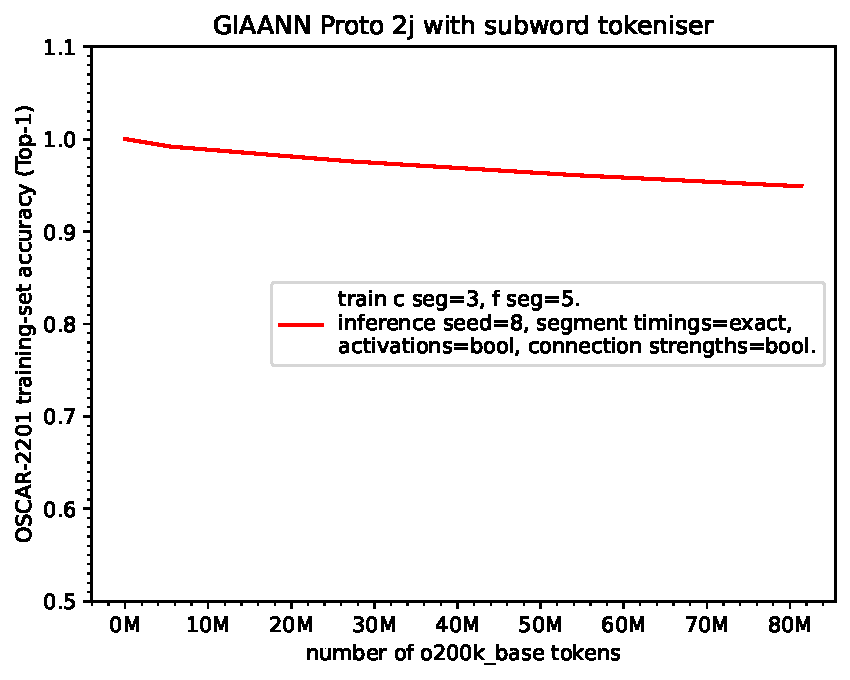
\includegraphics[width=0.80\linewidth]{graphs/protov2j-oscar-train-top1-accuracy-spacyPipelineOptimisations-inferenceConnectionStrengthTypes.pdf}
      \caption{GIAANN Proto 2j training-set accuracy.}
      \label{fig:protov2j-oscar-train-top1-accuracy-spacyPipelineOptimisations-inferenceConnectionStrengthTypes}
\end{figure}

\begin{figure}[p]
      \centering
      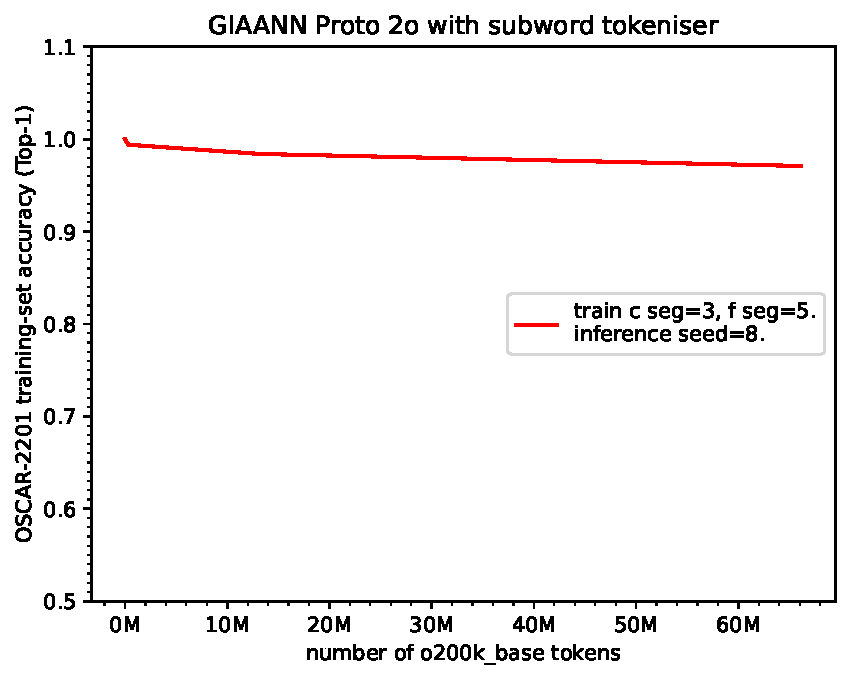
\includegraphics[width=0.80\linewidth]{graphs/protov2o-oscar-train-top1-accuracy-spacyPipelineOptimisations-inferenceConnectionStrengthTypes.pdf}
      \caption{GIAANN Proto 2o training-set accuracy.}
      \label{fig:protov2o-oscar-train-top1-accuracy-spacyPipelineOptimisations-inferenceConnectionStrengthTypes}
\end{figure}

\clearpage

\subsubsection{Test-set Accuracy}

\paragraph{Tables}

\Cref{tab:protov2j-oscar-test-top1-accuracy-spacyPipelineOptimisations-inferenceConnectionStrengthTypes} contains Proto v2j OSCAR-2201 Top-1 test-set accuracy for different inference connection strength types, training sizes, and inference activations, with segment timing none (t-1 none), targets fed as input, and multi-sentence predictions disabled. The different inference connection strength types used were ``bool'' (\texttt{inferenceConnectionsStrengthBoolean=True}) and ``float'' (\texttt{inferenceConnectionsStrengthBoolean=False}). The default segment timings used during proto v2j benchmarking is ``none''. The default inference activation type used during proto v2j benchmarking is ``bool f''. The default strength type used during proto v2j benchmarking is ``float''. The table also includes the total number of trained words and tokens. 

\Cref{tab:protov2k-oscar-test-top1-accuracy} contains Proto v2k OSCAR-2201 Top-1 test-set accuracy for different training sizes, with targets fed as input, and multi-sentence predictions disabled. The default segment timings used during proto v2k benchmarking is ``biased''. The default inference activation type used during proto v2k benchmarking is ``int c+f''. The default strength type used during proto v2k benchmarking is ``float''. \texttt{inferenceActivationFunction} was also disabled during proto v2k benchmarking. The table also includes the total number of trained words and tokens. 

\Cref{tab:protov2k-oscar-test-top1-accuracy-multisentencePredictions} contains Proto v2k OSCAR-2201 Top-1 test-set accuracy for different training sizes, and with targets fed as input.

\Cref{tab:protov2m-oscar-test-top1-accuracy-inferenceLeakyIntegrateAndFire} contains Proto v2m OSCAR-2201 Top-1 test-set accuracy for different training sizes, with targets fed as input. The table also includes the total number of trained words and tokens.

\Cref{tab:protov2m-oscar-test-top1-accuracy-segmentSizes-inferenceLeakyIntegrateAndFire} contains Proto v2m OSCAR-2201 Top-1 test-set accuracy for different numbers of segments, with targets fed as input

\Cref{tab:protov2m-oscar-test-top1-accuracy-models-inferenceLeakyIntegrateAndFire} contains Proto v2m OSCAR-2201 Top-1 test-set accuracy for different training sizes and models, with targets fed as input. \texttt{sentencePredictions=False} was set to generate similar context window sizes for the comparison.

\Cref{tab:protov2o-oscar-test-top1-accuracy-inferenceLeakyIntegrateAndFire} contains Proto v2o OSCAR-2201 Top-1 test-set accuracy for different training sizes, with targets fed as input. The table also includes the total number of trained words and tokens.

\Cref{tab:protov2o-oscar-test-top1-accuracy-models-inferenceLeakyIntegrateAndFire} contains Proto v2o OSCAR-2201 Top-1 test-set accuracy for different training sizes and models, with targets fed as input. \texttt{sentencePredictions=False} was set to generate similar context window sizes for the comparison.

\Cref{tab:protov2o-oscar-test-top1-accuracy-models-inferenceLeakyIntegrateAndFire-predictionEnsureConnectedToPreviousPredictionTrue} contains Proto v2o OSCAR-2201 Top-1 test-set accuracy for different training sizes and models, with targets fed as input, and \texttt{predictionEnsureConnectedToPreviousPrediction=True}. \texttt{sentencePredictions=False} was set to generate similar context window sizes for the comparison.

\Cref{tab:protov2o-oscar-test-top1-accuracy-models-inferenceLeakyIntegrateAndFire-predictionEnsureConnectedToPreviousPredictionFalse} contains Proto v2o OSCAR-2201 Top-1 test-set accuracy for different training sizes and models, with targets fed as input, and and \texttt{predictionEnsureConnectedToPreviousPrediction=alse}. \texttt{sentencePredictions=False} was set to generate similar context window sizes for the comparison.

\Cref{fig:protov2j-oscar-test-top1-accuracy-spacyPipelineOptimisations-inferenceConnectionStrengthTypes} graphs the v2j test-set eval results.

\Cref{fig:protov2o-oscar-test-top1-accuracy-spacyPipelineOptimisations-inferenceConnectionStrengthTypes} graphs the v2o test-set eval results.

An additional set of results were created with \texttt{sentencePredictions=False} to generate similar context window sizes (i.e. context window size sentence independence) for the comparison with a 6-layer 512-token context RoBERTa Causal Transformer Language Model \citep{liu2019roberta} executed within TSBNLP \citep{bairesearch2022TSBNLP}.


\begin{table}[H]
\centering
\caption{Proto v2j OSCAR-2201 Top-1 test-set accuracy for different inference connection strength types, training sizes, and inference activations, with segment timing none (t-1 none), targets fed as input, and multi-sentence predictions disabled.}
\label{tab:protov2j-oscar-test-top1-accuracy-spacyPipelineOptimisations-inferenceConnectionStrengthTypes}
\begin{tabular}{rrrrrrrrrrr}
\toprule
\textbf{s} & \textbf{c} & \textbf{f} & \textbf{sequences} & \textbf{str} & \textbf{int f+c} & \textbf{bool f} & \textbf{param} & \textbf{db size} & \textbf{words} & \textbf{tokens} \\
\midrule
8 & 3 & 5 & 5,000     & bool & 0.073 & 0.068 & 1.0M & 0.2GB & 0.1M & 0.1M \\
8 & 3 & 5 & 200,000   & bool & 0.178 & 0.182 & 34.0M & 3.9GB & 5.0M & 5.5M \\
8 & 3 & 5 & 1,000,000 & bool & 0.227 & 0.225 & 157.0M & 15.0GB & 24.6M & 27.1M \\
8 & 3 & 5 & 2,000,000 & bool & 0.237 & 0.230 & 296.4M & 26.2GB & 49.2M & 54.3M \\
8 & 3 & 5 & 3,000,000 & bool & 0.238 & 0.230 & 433.5M & 36.8GB & 73.8M & 81.4M \\
8 & 3 & 5 & 5,000     & float & 0.078 & 0.074 & 1.0M & 0.2GB & 0.1M & 0.1M \\
8 & 3 & 5 & 200,000   & float & 0.205 & 0.192 & 34.0M & 3.9GB & 5.0M & 5.5M \\
8 & 3 & 5 & 1,000,000 & float & 0.238 & 0.237 & 157.0M & 15.0GB & 24.6M & 27.1M \\
8 & 3 & 5 & 2,000,000 & float & 0.253 & 0.253 & 296.4M & 26.2GB & 49.2M & 54.3M \\
8 & 3 & 5 & 3,000,000 & float & 0.256 & 0.262 & 433.5M & 36.8GB & 73.8M & 81.4M \\
\bottomrule
\end{tabular}
\end{table}

\begin{table}[H]
\centering
\caption{Proto v2k OSCAR-2201 Top-1 test-set accuracy for different training sizes, with targets fed as input, and multi-sentence predictions disabled.}
\label{tab:protov2k-oscar-test-top1-accuracy}
\begin{tabular}{rrrrrrrrrrr}
\toprule
\textbf{s} & \textbf{c} & \textbf{f} & \textbf{sequences} & \textbf{t-1} & \textbf{param} & \textbf{db size} & \textbf{words} & \textbf{tokens} \\
\midrule
8 & 3 & 5 & 5,000     & 0.065 & 2.0M & 0.3GB & 0.1M & 0.1M \\
8 & 3 & 5 & 200,000   & 0.167 & 74.9M & 7.4GB &	5.2M & 5.8M \\
8 & 3 & 5 & 1,000,000 & 0.192 & 347.0M & 29.3GB & 26.0M & 28.8M \\
\bottomrule
\end{tabular}
\end{table}

\begin{table}[H]
\centering
\caption{Proto v2k OSCAR-2201 Top-1 test-set accuracy for different training sizes, with targets fed as input.}
\label{tab:protov2k-oscar-test-top1-accuracy-multisentencePredictions}
\begin{tabular}{rrrrrrrrrrr}
\toprule
\textbf{s} & \textbf{c} & \textbf{f} & \textbf{sequences} & \textbf{t-1} & \textbf{param} & \textbf{db size} & \textbf{words} & \textbf{tokens} \\
\midrule
8 & 3 & 5 & 5,000     & 0.081 & 5.8M & 0.7GB & 0.3M & 0.3M \\
8 & 3 & 5 & 200,000   & 0.164 & 212.3M & 17.2GB & 11.9M & 13.2M \\
8 & 3 & 5 & 1,000,000 & 0.189 & 979.4M & 69.9GB & 59.6M & 66.2M \\
\bottomrule
\end{tabular}
\end{table}

\begin{table}[H]
\centering
\caption{Proto v2m OSCAR-2201 Top-1 test-set accuracy for different training sizes, with targets fed as input.}
\label{tab:protov2m-oscar-test-top1-accuracy-inferenceLeakyIntegrateAndFire}
\begin{tabular}{rrrrrrrrr}
\toprule
\textbf{s} & \textbf{c} & \textbf{f} & \textbf{sequences} & \textbf{t-1} & \textbf{param} & \textbf{db size} & \textbf{words} & \textbf{tokens} \\
\midrule
8 & 4 & 4 & 5,000     & 0.083 & 6.0M & 0.7GB & 0.3M & 0.3M \\
8 & 4 & 4 & 200,000   & 0.175 & 217.0M & 17.4GB & 11.9M & 13.2M \\
8 & 4 & 4 & 1,000,000 & 0.207 & 1000.7M & 69.5GB & 60.0M & 66.2M \\
\bottomrule
\end{tabular}
\end{table}

\begin{table}[H]
\centering
\caption{Proto v2m OSCAR-2201 Top-1 test-set accuracy for different numbers of segments, with targets fed as input.}
\label{tab:protov2m-oscar-test-top1-accuracy-segmentSizes-inferenceLeakyIntegrateAndFire}
\begin{tabular}{rrrrrrrrrr}
\toprule
\textbf{s} & \textbf{c} & \textbf{f} & \textbf{sequences} & \textbf{t-1} & \textbf{param} & \textbf{db size} & \textbf{words} & \textbf{tokens} \\
\midrule
8  & 4  & 4  & 200,000 & 0.175 & 217.0M & 17.4GB & 11.9M & 13.2M \\
16 & 8  & 8  & 200,000 & 0.176 & 391.7M & 25.4GB & 12.1M & 13.4M \\
32 & 16 & 16 & 200,000 & 0.182 & 611.4M & 36.1GB & 12.8M & 14.2M \\
\bottomrule
\end{tabular}
\end{table}

\begin{table}[H]
\centering
\caption{Proto v2m OSCAR-2201 Top-1 test-set accuracy for different training sizes and models, with targets fed as input.}
\label{tab:protov2m-oscar-test-top1-accuracy-models-inferenceLeakyIntegrateAndFire}
\begin{tabular}{rrrrrrrrrr}
\toprule
\textbf{s} & \textbf{c} & \textbf{f} & \textbf{sequences} & \textbf{model} & \textbf{t-1} & \textbf{param} & \textbf{db size} & \textbf{words} & \textbf{tokens} \\
\midrule
8 & 4 & 4 & 10,000  & GIAANN & 0.156 & 71.2M & 6.0GB & 3.4M & 3.8M \\
8 & 4 & 4 & 100,000 & GIAANN & 0.233 & 657.6M & 45.7GB & 33.3M & 37.5M \\
- & - & - & 10,000  & RoBERTa & 0.147 & 67.3M & 257.1MB & 2.4M & 3.2M \\
- & - & - & 100,000 & RoBERTa & 0.316 & 67.3M & 257.1MB & 24.3M & 32.9M \\
\bottomrule
\end{tabular}
\end{table}

\begin{table}[H]
\centering
\caption{Proto v2o OSCAR-2201 Top-1 test-set accuracy for different training sizes, with targets fed as input.}
\label{tab:protov2o-oscar-test-top1-accuracy-inferenceLeakyIntegrateAndFire}
\begin{tabular}{rrrrrrrrr}
\toprule
\textbf{s} & \textbf{c} & \textbf{f} & \textbf{sequences} & \textbf{t-1} & \textbf{param} & \textbf{db size} & \textbf{words} & \textbf{tokens} \\
\midrule
8 & 4 & 4 & 5,000     & 0.097 & 6.0M & 0.7GB & 0.3M & 0.3M  \\
8 & 4 & 4 & 200,000   & 0.189 & 217.0M  & 17.4GB & 11.9M & 13.2M \\
8 & 4 & 4 & 1,000,000 & 0.217 & 1000.7M & 69.5GB & 60.0M & 66.2M \\
\bottomrule
\end{tabular}
\end{table}

\begin{table}[H]
\centering
\caption{Proto v2o OSCAR-2201 Top-1 test-set accuracy for different training sizes and models, with targets fed as input.}
\label{tab:protov2o-oscar-test-top1-accuracy-models-inferenceLeakyIntegrateAndFire}
\begin{tabular}{rrrrrrrrrr}
\toprule
\textbf{s} & \textbf{c} & \textbf{f} & \textbf{sequences} & \textbf{model} & \textbf{t-1} & \textbf{param} & \textbf{db size} & \textbf{words} & \textbf{tokens} \\
\midrule
8 & 4 & 4 & 10,000  & GIAANN & 0.173 & 71.2M & 6.0GB & 3.4M & 3.8M \\
8 & 4 & 4 & 100,000 & GIAANN & 0.250 & 657.6M & 45.7GB & 33.3M & 37.5M \\
- & - & - & 10,000  & RoBERTa & 0.147 & 67.3M & 257.1MB & 2.4M & 3.2M \\
- & - & - & 100,000 & RoBERTa & 0.316 & 67.3M & 257.1MB & 24.3M & 32.9M \\
\bottomrule
\end{tabular}
\end{table}

%FUTURE:
\begin{table}[H]
\centering
\caption{Proto v2o OSCAR-2201 Top-1 test-set accuracy for different training sizes and models, with targets fed as input, and \texttt{predictionEnsureConnectedToPreviousPrediction=True}.}
\label{tab:protov2o-oscar-test-top1-accuracy-models-inferenceLeakyIntegrateAndFire-predictionEnsureConnectedToPreviousPredictionTrue}
\begin{tabular}{rrrrrrrrrr}
\toprule
\textbf{s} & \textbf{c} & \textbf{f} & \textbf{sequences} & \textbf{model} & \textbf{t-1} & \textbf{param} & \textbf{db size} & \textbf{words} & \textbf{tokens} \\
\midrule
8 & 4 & 4 & 10,000  & GIAANN & 0.168 & 71.2M & 6.0GB & 3.4M & 3.8M \\
8 & 4 & 4 & 100,000 & GIAANN & 0.269 & 657.6M & 45.7GB & 33.3M & 37.5M \\
- & - & - & 10,000  & RoBERTa & 0.152 & 67.3M & 257.1MB & 2.4M & 3.2M \\
- & - & - & 100,000 & RoBERTa & 0.317 & 67.3M & 257.1MB & 24.3M & 32.9M \\
\bottomrule
\end{tabular}
\end{table}

\begin{table}[H]
\centering
\caption{Proto v2o OSCAR-2201 Top-1 test-set accuracy for different training sizes and models, with targets fed as input, and \texttt{predictionEnsureConnectedToPreviousPrediction=False}.}
\label{tab:protov2o-oscar-test-top1-accuracy-models-inferenceLeakyIntegrateAndFire-predictionEnsureConnectedToPreviousPredictionFalse}
\begin{tabular}{rrrrrrrrrr}
\toprule
\textbf{s} & \textbf{c} & \textbf{f} & \textbf{sequences} & \textbf{model} & \textbf{t-1} & \textbf{param} & \textbf{db size} & \textbf{words} & \textbf{tokens} \\
\midrule
8 & 4 & 4 & 10,000  & GIAANN & 0.212 & 71.2M & 6.0GB & 3.4M & 3.8M \\
8 & 4 & 4 & 100,000 & GIAANN & 0.297 & 657.6M & 45.7GB & 33.3M & 37.5M \\
- & - & - & 10,000  & RoBERTa & 0.152 & 67.3M & 257.1MB & 2.4M & 3.2M \\
- & - & - & 100,000 & RoBERTa & 0.317 & 67.3M & 257.1MB & 24.3M & 32.9M \\
\bottomrule
\end{tabular}
\end{table}

\clearpage

\begin{figure}[p]
      \centering
      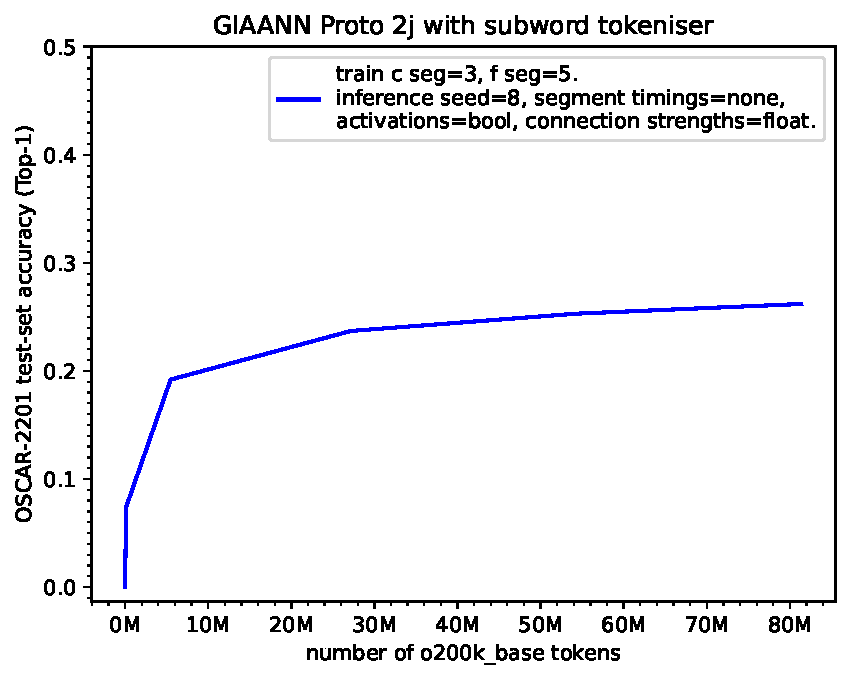
\includegraphics[width=0.80\linewidth]{graphs/protov2j-oscar-test-top1-accuracy-spacyPipelineOptimisations-inferenceConnectionStrengthTypes.pdf}
      \caption{GIAANN Proto 2j test-set accuracy.}
      \label{fig:protov2j-oscar-test-top1-accuracy-spacyPipelineOptimisations-inferenceConnectionStrengthTypes}
\end{figure}

\begin{figure}[p]
      \centering
      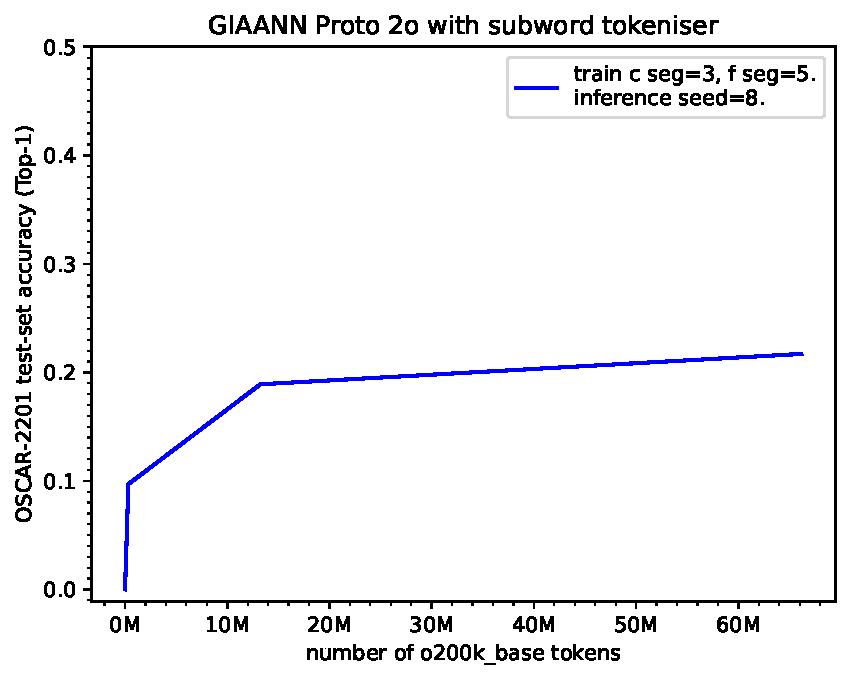
\includegraphics[width=0.80\linewidth]{graphs/protov2o-oscar-test-top1-accuracy-spacyPipelineOptimisations-inferenceConnectionStrengthTypes.pdf}
      \caption{GIAANN Proto 2o test-set accuracy.}
      \label{fig:protov2o-oscar-test-top1-accuracy-spacyPipelineOptimisations-inferenceConnectionStrengthTypes}
\end{figure}

\clearpage

\subsection{Performance (proto v2)}

An additional set of performance measurements were taken with GIAANN Proto 2.

A number of optimisations were introduced in GIAANN Proto 2 that affect evaluation performance:

\begin{itemize}
 	\item perf(eval): vectorize SANI required-segment candidate filtering
			- replace Python set/list membership checks in prediction candidate filtering with tensor key membership. This keeps SANI required-segment semantics unchanged while avoiding per-candidate Python loops during long eval sequences.
 	\item perf(eval): prefilter sparse candidate aggregation by required segment keys
			- push required SANI column-feature key filtering into sparse aggregation so irrelevant activation entries are removed before branch reduction and candidate aggregation.
 	\item perf(sparse): vectorize sparse branch max reduction
			- replace Python grouping loops in \texttt{reduceSparseBranchMax()} with tensor \texttt{unique}/\texttt{scatter_reduce_} operations. This improves multiple-branch sparse activation reduction used during inference candidate selection.
 	\item perf(sparse): replace broadcast sparse intersection with key lookup
			- rework \texttt{selectAindicesContainedInB()} to use flattened sparse index keys and \texttt{searchsorted} membership instead of an $O(nnzA * nnzB)$ broadcast comparison.
 	\item perf(eval): avoid full coalesce in sparse branch selection
			- optimise \texttt{selectActivatedBranchIndex()} by using sparse \texttt{_indices()}/\texttt{_values()} and tensor \texttt{index_add_} for branch scoring, avoiding full tensor coalescing and Python dictionaries during prediction deactivation.
\end{itemize}

All proto v2 performance measurements were conducted with different database feature connections active storage location for train/eval (DDR5 RAM/filesystem), with train phase feature neuron and connection sparse tensors, sparse tensor device CPU, and feature neuron sparse tensors stored independently for each column. 

\texttt{optimisationStoreDatabaseResidentCoordinatesAsInt32=True} was set during all proto v2m+ training rounds to reduce RAM usage. 

\paragraph{Tables}

\Cref{tab:protov2j-oscar-performance} contains Proto v2j OSCAR-2201 performance measurements for different execution phases (train, eval test-set) and training sizes and different training sizes, with multi-sentence predictions disabled. Train times were measured cumulatively > 1M sequences.

\Cref{tab:protov2k-oscar-performance} contains Proto v2k OSCAR-2201 performance measurements for different execution phases (train, eval training-set, eval test-set) and training sizes, with multi-sentence predictions disabled.

\Cref{tab:protov2k-oscar-performance-multisentencePredictions} contains Proto v2k OSCAR-2201 performance measurements for different execution phases (train, eval training-set, eval test-set) and training sizes and different training sizes.

\Cref{tab:protov2m-oscar-performance-inferenceLeakyIntegrateAndFire} contains Proto v2m OSCAR-2201 performance measurements for different execution phases (train, eval training-set, eval test-set) and training sizes.

\Cref{tab:protov2m-oscar-performance-segmentSizes-inferenceLeakyIntegrateAndFire} contains Proto v2m OSCAR-2201 performance measurements for different execution phases (train, eval training-set, eval test-set) and numbers of segments.

\Cref{tab:protov2m-oscar-performance-models-inferenceLeakyIntegrateAndFire} contains Proto v2m OSCAR-2201 performance measurements for different training sizes, models and execution phases (train, eval test-set). TSBNLP was executed on device GPU.

\Cref{tab:protov2o-oscar-performance-inferenceLeakyIntegrateAndFire} contains proto v2o OSCAR-2201 performance measurements for different execution phases (train, eval training-set, eval test-set) and training sizes.

\Cref{tab:protov2o-oscar-performance-models-inferenceLeakyIntegrateAndFire} contains Proto v2o OSCAR-2201 performance measurements for different training sizes, models and execution phases (train, eval test-set). TSBNLP was executed on device GPU.

\begin{table}[H]
\centering
\caption{Proto v2j OSCAR-2201 performance measurements for different execution phases (train, eval test-set) and training sizes, with multi-sentence predictions disabled.}
\label{tab:protov2j-oscar-performance}
\begin{tabular}{rrrrrrrrrrrr}
\toprule
\textbf{s} & \textbf{c} & \textbf{f} & \textbf{sequences} & \textbf{phase} & \textbf{t tot} & \textbf{t proc} & \textbf{t w/r} & \textbf{cpu ram} \\
\midrule
8 & 3 & 5 & 5,000       & train   & 00:00:32 & 00:00:27 & 00:00:05 & 1.4GB \\
8 & 3 & 5 & 200,000     & train   & 00:25:09 & 00:23:31 & 00:01:37 & 5.6GB \\
8 & 3 & 5 & 1,000,000   & train   & 02:53:06 & 02:47:08 & 00:05:57 & 18.7GB \\
8 & 3 & 5 & 2,000,000   & train   & 08:10:49 & 07:23:41 & 00:11:10 & 31.9GB \\
8 & 3 & 5 & 3,000,000   & train   & 18:54:29 & 16:40:48 & 00:17:03 & 44.9GB \\
8 & 3 & 5 & 5,000       & ts eval & 00:00:02 & 00:00:02 & 00:00:00 & 1.1GB \\
8 & 3 & 5 & 200,000     & ts eval & 00:00:04 & 00:00:04 & 00:00:00 & 1.1GB \\
8 & 3 & 5 & 1,000,000   & ts eval & 00:00:11 & 00:00:11 & 00:00:00 & 1.1GB \\
8 & 3 & 5 & 2,000,000   & ts eval & 00:00:16 & 00:00:16 & 00:00:00 & 1.1GB \\
8 & 3 & 5 & 3,000,000   & ts eval & 00:00:21 & 00:00:21 & 00:00:00 & 1.1GB \\
\bottomrule
\end{tabular}
\end{table}

\begin{table}[H]
\centering
\caption{Proto v2k OSCAR-2201 performance measurements for different execution phases (train, eval training-set, eval test-set) and training sizes, with multi-sentence predictions disabled.}
\label{tab:protov2k-oscar-performance}
\begin{tabular}{rrrrrrrrrrrr}
\toprule
\textbf{s} & \textbf{c} & \textbf{f} & \textbf{sequences} & \textbf{phase} & \textbf{t tot} & \textbf{t proc} & \textbf{t w/r} & \textbf{cpu ram} \\
\midrule
8 & 3 & 5 & 5,000       & train   & 00:00:50 & 00:00:42 & 00:00:07 & 1.4GB \\
8 & 3 & 5 & 200,000     & train   & 00:56:46 & 00:54:05 & 00:02:40 & 7.9GB \\
8 & 3 & 5 & 1,000,000   & train   & 05:56:15 & 05:46:32 & 00:09:43 & 31.1GB \\
8 & 3 & 5 & 5,000       & tr eval & 00:01:07 & 00:01:07 & 00:00:00 & 1.2GB \\
8 & 3 & 5 & 200,000     & tr eval & 00:02:38 & 00:02:38 & 00:00:00 & 1.2GB \\
8 & 3 & 5 & 1,000,000   & tr eval & 00:06:24 & 00:06:24 & 00:00:00 & 1.3GB \\
8 & 3 & 5 & 5,000       & ts eval & 00:00:39 & 00:00:39 & 00:00:00 & 1.2GB \\
8 & 3 & 5 & 200,000     & ts eval & 00:02:29 & 00:02:29 & 00:00:00 & 1.2GB \\
8 & 3 & 5 & 1,000,000   & ts eval & 00:06:28 & 00:06:28 & 00:00:00 & 1.3GB \\
\bottomrule
\end{tabular}
\end{table}

\begin{table}[H]
\centering
\caption{Proto v2k OSCAR-2201 performance measurements for different execution phases (train, eval training-set, eval test-set) and training sizes.}
\label{tab:protov2k-oscar-performance-multisentencePredictions}
\begin{tabular}{rrrrrrrrrrrr}
\toprule
\textbf{s} & \textbf{c} & \textbf{f} & \textbf{sequences} & \textbf{phase} & \textbf{t tot} & \textbf{t proc} & \textbf{t w/r} & \textbf{cpu ram} \\
\midrule
8 & 3 & 5 & 5,000       & train   & 00:01:45 & 00:01:28 & 00:00:16 & 1.8GB \\
8 & 3 & 5 & 200,000     & train   & 02:02:06 & 01:56:42 & 00:05:24 & 17.9GB \\
8 & 3 & 5 & 1,000,000   & train   & - & - & - & - \\
8 & 3 & 5 & 5,000       & tr eval & 00:02:41 & 00:02:41 & 00:00:00 & 1.3GB \\
8 & 3 & 5 & 200,000     & tr eval & 00:14:36 & 00:14:36 & 00:00:00 & 1.3GB \\
8 & 3 & 5 & 1,000,000   & tr eval & 00:51:26 & 00:51:26 & 00:00:00 & 1.6GB \\
8 & 3 & 5 & 5,000       & ts eval & 00:02:34 & 00:02:34 & 00:00:00 & 1.3GB \\
8 & 3 & 5 & 200,000     & ts eval & 00:16:35 & 00:16:35 & 00:00:00 & 1.4GB \\
8 & 3 & 5 & 1,000,000   & ts eval & 00:51:00 & 00:51:00 & 00:00:00 & 1.7GB \\
\bottomrule
\end{tabular}
\end{table}

\begin{table}[H]
\centering
\caption{Proto v2m OSCAR-2201 performance measurements for different execution phases (train, eval training-set, eval test-set) and training sizes.}
\label{tab:protov2m-oscar-performance-inferenceLeakyIntegrateAndFire}
\begin{tabular}{rrrrrrrrr}
\toprule
\textbf{s} & \textbf{c} & \textbf{f} & \textbf{sequences} & \textbf{phase} & \textbf{t tot} & \textbf{t proc} & \textbf{t w/r} & \textbf{cpu ram} \\
\midrule
8 & 4 & 4 & 5,000       & train   & 00:01:56 & 00:01:36 & 00:00:19 & 1.6GB \\
8 & 4 & 4 & 200,000     & train   & 02:35:53 & 02:29:07 & 00:06:45 & 12.7GB \\
8 & 4 & 4 & 1,000,000   & train   & 44:34:27 & 43:14:01 & 01:20:26 & 55.3GB \\
8 & 4 & 4 & 5,000       & tr eval & 00:02:11 & 00:02:11 & 00:00:00 & 1.3GB \\
8 & 4 & 4 & 200,000     & tr eval & 00:08:00 & 00:08:00 & 00:00:00 & 1.3GB \\
8 & 4 & 4 & 1,000,000   & tr eval & 00:21:02 & 00:21:02 & 00:00:00 & 1.5GB \\
8 & 4 & 4 & 5,000       & ts eval & 00:02:10 & 00:02:10 & 00:00:00 & 1.3GB \\
8 & 4 & 4 & 200,000     & ts eval & 00:17:14 & 00:17:14 & 00:00:00 & 1.3GB \\
8 & 4 & 4 & 1,000,000   & ts eval & 00:49:05 & 00:49:05 & 00:00:00 & 1.6GB \\
\bottomrule
\end{tabular}
\end{table}

\begin{table}[H]
\centering
\caption{Proto v2m OSCAR-2201 performance measurements for different execution phases (train, eval training-set, eval test-set) and numbers of segments.}
\label{tab:protov2m-oscar-performance-segmentSizes-inferenceLeakyIntegrateAndFire}
\begin{tabular}{rrrrrrrrr}
\toprule
\textbf{s} & \textbf{c} & \textbf{f} & \textbf{sequences} & \textbf{phase} & \textbf{t tot} & \textbf{t proc} & \textbf{t w/r} & \textbf{cpu ram} \\
\midrule
8 & 4 & 4 & 200,000     & train   & 02:35:53 & 02:29:07 & 00:06:45 & 12.7GB \\
16 & 8 & 8 & 200,000    & train   & 03:44:16 & 03:36:13 & 00:08:03 & 18.3GB \\
32 & 16 & 16 & 200,000  & train   & 05:12:34 & 05:05:12 & 00:07:21 & 27.1GB \\
8 & 4 & 4 & 200,000     & tr eval & 00:08:00 & 00:08:00 & 00:00:00 & 1.3GB \\
16 & 8 & 8 & 200,000    & tr eval & 00:13:15 & 00:13:15 & 00:00:00 & 1.3GB \\
32 & 16 & 16 & 200,000  & tr eval & 00:18:43 & 00:18:43 & 00:00:00 & 1.4GB \\
8 & 4 & 4 & 200,000     & ts eval & 00:17:14 & 00:17:14 & 00:00:00 & 1.3GB \\
16 & 8 & 8 & 200,000    & ts eval & 00:24:22 & 00:24:22 & 00:00:00 & 1.4GB \\
32 & 8 & 8 & 200,000    & ts eval & 00:33:43 & 00:33:43 & 00:00:00 & 1.5GB \\
\bottomrule
\end{tabular}
\end{table}

\begin{table}[H]
\centering
\caption{Proto v2m OSCAR-2201 performance measurements for different training sizes, models and execution phases (train, eval test-set).}
\label{tab:protov2m-oscar-performance-models-inferenceLeakyIntegrateAndFire}
\begin{tabular}{rrrrrrr}
\toprule
\textbf{s} & \textbf{c} & \textbf{f} & \textbf{sequences} & \textbf{model} & \textbf{phase} & \textbf{t tot} \\
\midrule
8 & 4 & 4 & 10,000  & GIAANN  & train   & 00:26:29 \\
8 & 4 & 4 & 100,000 & GIAANN  & train   & 10:51:45 \\
- & - & - & 10,000  & RoBERTa & train   & 00:04:09 \\
- & - & - & 100,000 & RoBERTa & train   & 00:40:58 \\
8 & 4 & 4 & 10,000  & GIAANN  & ts eval & 02:05:30 \\
8 & 4 & 4 & 100,000 & GIAANN  & ts eval & 09:28:27 \\
- & - & - & 10,000  & RoBERTa & ts eval & 00:03:13 \\
- & - & - & 100,000 & RoBERTa & ts eval & 00:02:59 \\
\bottomrule
\end{tabular}
\end{table}


\begin{table}[H]
\centering
\caption{Proto v2o OSCAR-2201 performance measurements for different execution phases (train, eval training-set, eval test-set) and training sizes.}
\label{tab:protov2o-oscar-performance-inferenceLeakyIntegrateAndFire}
\begin{tabular}{rrrrrrrrr}
\toprule
\textbf{s} & \textbf{c} & \textbf{f} & \textbf{sequences} & \textbf{phase} & \textbf{t tot} & \textbf{t proc} & \textbf{t w/r} & \textbf{cpu ram} \\
\midrule
8 & 4 & 4 & 5,000       & train   & 00:01:59 & 00:01:40 & 00:00:19 & 1.6GB \\
8 & 4 & 4 & 200,000     & train   & 02:36:04 & 02:29:04 & 00:07:00 & 12.7GB \\
8 & 4 & 4 & 1,000,000   & train   & 36:01:34 & 34:53:14 & 01:08:20 & 54.6GB \\
8 & 4 & 4 & 5,000       & tr eval & 00:01:50 & 00:01:50 & 00:00:00 & 1.3GB \\
8 & 4 & 4 & 200,000     & tr eval & 00:08:28 & 00:08:28 & 00:00:00 & 1.3GB \\
8 & 4 & 4 & 1,000,000   & tr eval & 00:31:44 & 00:31:44 & 00:00:00 & 1.5GB \\
8 & 4 & 4 & 5,000       & ts eval & 00:02:13 & 00:02:13 & 00:00:00 & 1.3GB \\
8 & 4 & 4 & 200,000     & ts eval & 00:19:20 & 00:19:20 & 00:00:00 & 1.3GB \\
8 & 4 & 4 & 1,000,000   & ts eval & 00:57:31 & 00:57:31 & 00:00:00 & 1.7GB \\
\bottomrule
\end{tabular}
\end{table}

\begin{table}[H]
\centering
\caption{Proto v2o OSCAR-2201 performance measurements for different training sizes, models and execution phases (train, eval training-set, eval test-set).}
\label{tab:protov2o-oscar-performance-models-inferenceLeakyIntegrateAndFire}
\begin{tabular}{rrrrrrr}
\toprule
\textbf{s} & \textbf{c} & \textbf{f} & \textbf{sequences} & \textbf{model} & \textbf{phase} & \textbf{t tot} \\
\midrule
8 & 4 & 4 & 10,000  & GIAANN  & train   & 00:34:26 \\
8 & 4 & 4 & 100,000 & GIAANN  & train   & 10:39:16 \\
- & - & - & 10,000  & RoBERTa & train   & 00:04:09 \\
- & - & - & 100,000 & RoBERTa & train   & 00:40:58 \\
8 & 4 & 4 & 10,000  & GIAANN  & tr eval & 00:46:28 \\
8 & 4 & 4 & 100,000 & GIAANN  & tr eval & 02:22:18 \\
- & - & - & 10,000  & RoBERTa & tr eval & 00:02:25 \\
- & - & - & 100,000 & RoBERTa & tr eval & 00:02:18 \\
8 & 4 & 4 & 10,000  & GIAANN  & ts eval & 02:47:27 \\
8 & 4 & 4 & 100,000 & GIAANN  & ts eval & 11:32:32 \\
- & - & - & 10,000  & RoBERTa & ts eval & 00:03:31 \\
- & - & - & 100,000 & RoBERTa & ts eval & 00:03:22 \\
\bottomrule
\end{tabular}
\end{table}